\documentclass[twoside,a4paper]{refart}
\usepackage{makeidx}
\usepackage{ifthen}
\usepackage{graphicx}
\usepackage{float}
\usepackage[portuguese]{babel}

\def\bs{\char'134 } % backslash in \tt font.
\newcommand{\ie}{i.\,e.,}
\newcommand{\eg}{e.\,g..}
\DeclareRobustCommand\cs[1]{\texttt{\char`\\#1}}

\title{Manual de Operação Linux CNC}
\author{Grupo 2 - Projeto de Máquina PMR3411 - 2024 \\
Vinicios de Andrade Cardozo \\
Gabriel Silva de Carvalho  \\
Douglas Oliveira de Carvalho \\
Versão 1.5}

\date{10 de novembro, 2024}
\emergencystretch1em  %

\pagestyle{myfootings}
\markboth{Manual de operação do torno}%
         {Manual de operação do torno}

\makeindex 

\setcounter{tocdepth}{2}

\begin{document}

\maketitle

\begin{abstract}
Por meio deste texto vamos apresentar de maneira resumida a operação básica do torno controlado pelo Linux CNC, levando em conta peculiaridades presentes no controlador em relação a outras opções mais comuns e também as advindas de escolhas que ficaram a cargo do grupo de programação do projeto.
\end{abstract}

\tableofcontents

\newpage


%%%%%%%%%%%%%%%%%%%%%%%%%%%%%%%%%%%%%%%%%%%%%%%%%%%%%%%%%%%%%%%%%%%%

\section{Procedimentos inicias}

Aqui trataremos dos passos iniciais para começar a operar a máquina, ou seja, passos a serem realizados antes mesmo que o botão de ligar seja ativado na interface gráfica do aplicativo do LinuxCNC. 

\subsection{Inicialização e login}

Antes de ligar o computador é recomendável verificar que o Joystick esteja acoplado em uma entrada USB, uma vez que o LinuxCNC pode apresentar problemas de varredura de periféricos, ou seja, ele pode não detectar dispositivos conectados após sua inicialização (apesar de que esse problema nunca se apresentou para o caso de pendrives).

O próximo passo é conectar a caixa de controle a \textbf{uma tomada de 220V} (na sala de laboratório essas tomadas tem cor vermelha), e então ligar a caixa. Note que a caixa deve ser ligada antes de se ligar o computador pelo mesmo problema de varredura anteriormente citado.

Com os passos anteriores feitos, o computador pode ser ligado. Para acessá-lo basta que se entre com o login: \textbf{alunopmr} e a senha: \textbf{pmrcnc}. 

A última coisa a se fazer antes de se abrir o aplicativo do LinuxCNC é abrir um terminal e executar o comando: \textbf{qjoypad} para inicializar a aplicação que irá receber os inputs do Joystick e convertê-los para comandos de teclado que o LinuxCNC compreende. 

\subsection{Preparação para carregar um código G}
Abra o aplicativo do LinuxCNC, selecionando a configuração correta para o torno que será utilizado. Abaixo, dois métodos para se selecionar a configuração correta:

\begin{figure}[H]
    \begin{center}
        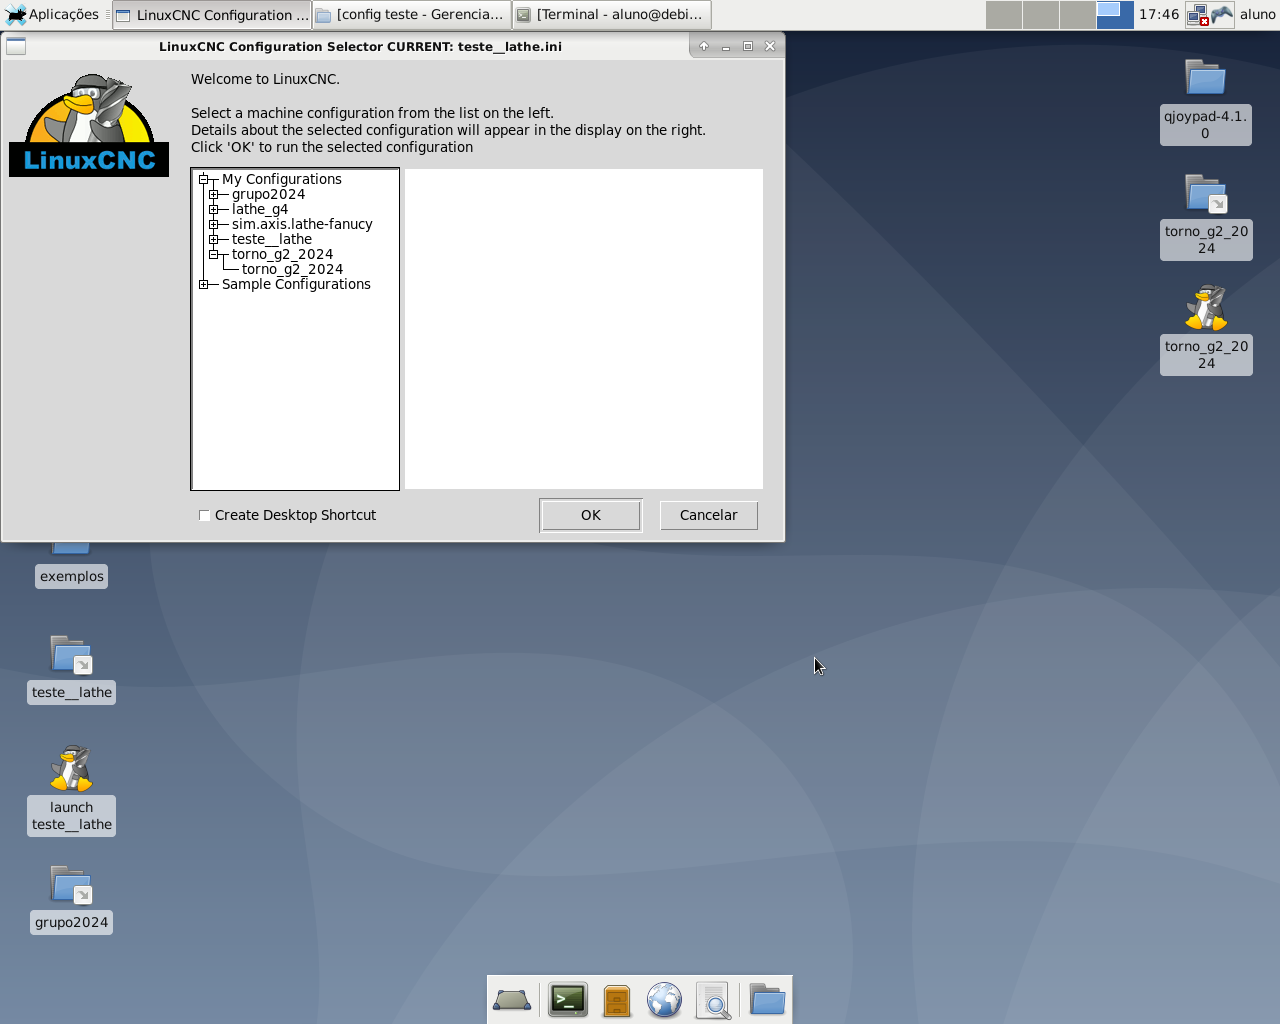
\includegraphics[width=0.95\textwidth]{imagens/Abertura_do_linux_CNC.png}
    \end{center}
    \caption{Seleção da configuração certa}\label{abrircncpiorjeito}
\end{figure}

\begin{figure}[H]
    \begin{center}
        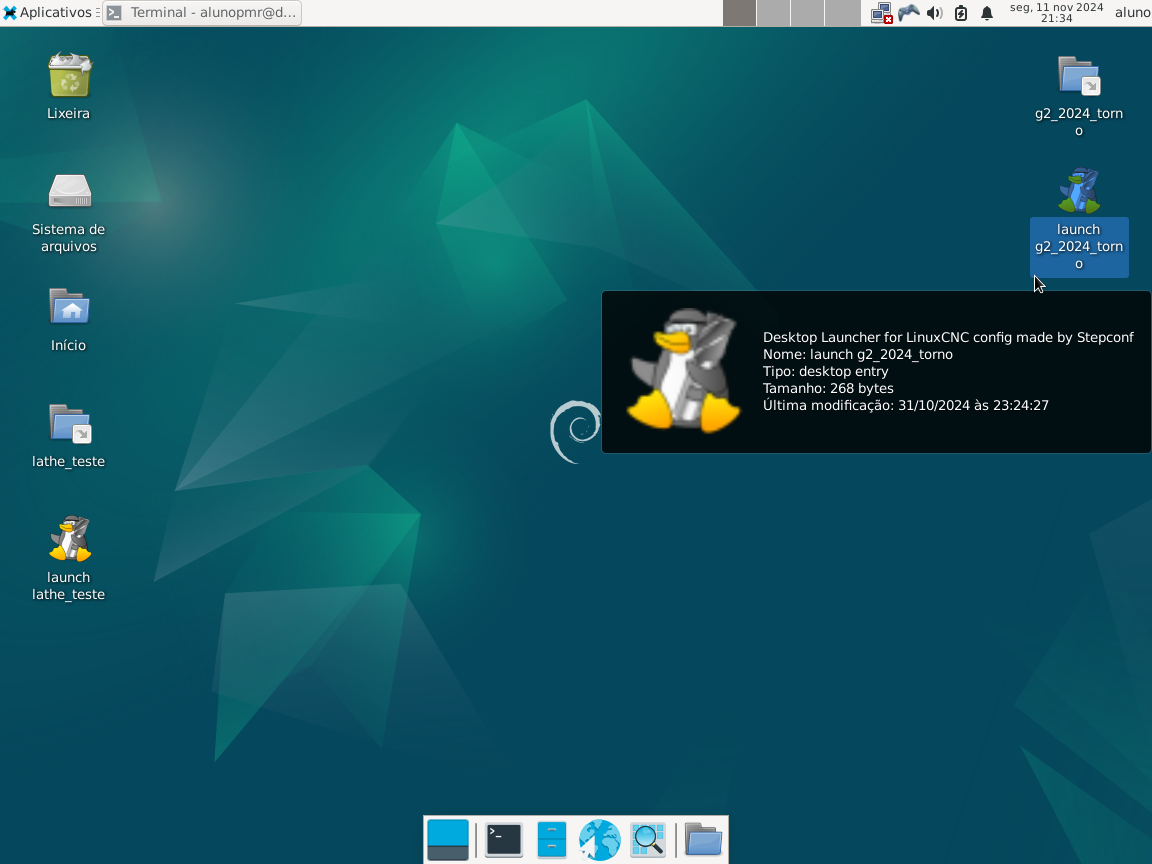
\includegraphics[width=0.95\textwidth]{imagens/atalho.png}
    \end{center}
    \caption{Abertura da configuração certa através de um atalho}\label{abrirmelhorjeito}
\end{figure}


Já com o aplicativo do LinuxCNC aberto, procure pelo botão vermelho de ligar no canto superior esquerdo da interface gráfica ou simplesmente utilize o botão "start" do Joystick, isso irá efetivamente ligar a máquina. 
Com o controle manual (Joystick ou teclado) leve o torno para uma posição segura e então faça o \textbf{homing} dos eixos X e Z.

\begin{figure}[H]
    \begin{center}
        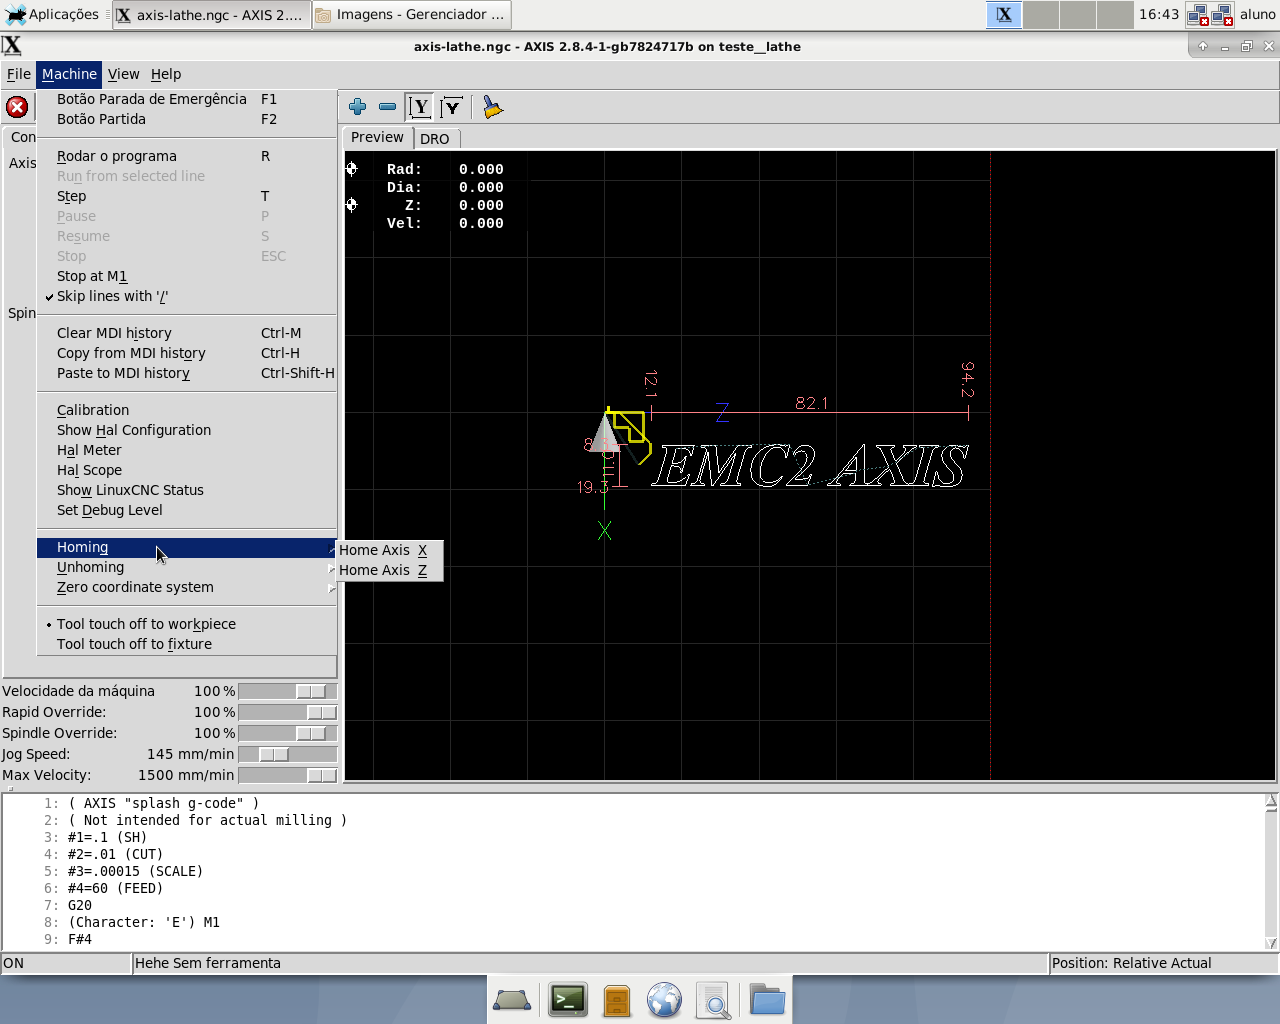
\includegraphics[width=0.95\textwidth]{imagens/referenciamento_linux_CNC.png}
    \end{center}
    \caption{Realização do homing}\label{homing}
\end{figure}


Para códigos G que descrevem diâmetros ao invés de raios (ou seja, códigos G usuais) é preciso que se ative o modo de diâmetro usando o comando G7 no MDI.

    Abra o código G da peça que você deseja produzir. Se houver algum erro na abertura modificações no código podem ser necessárias.

\begin{figure}[H]
    \begin{center}
        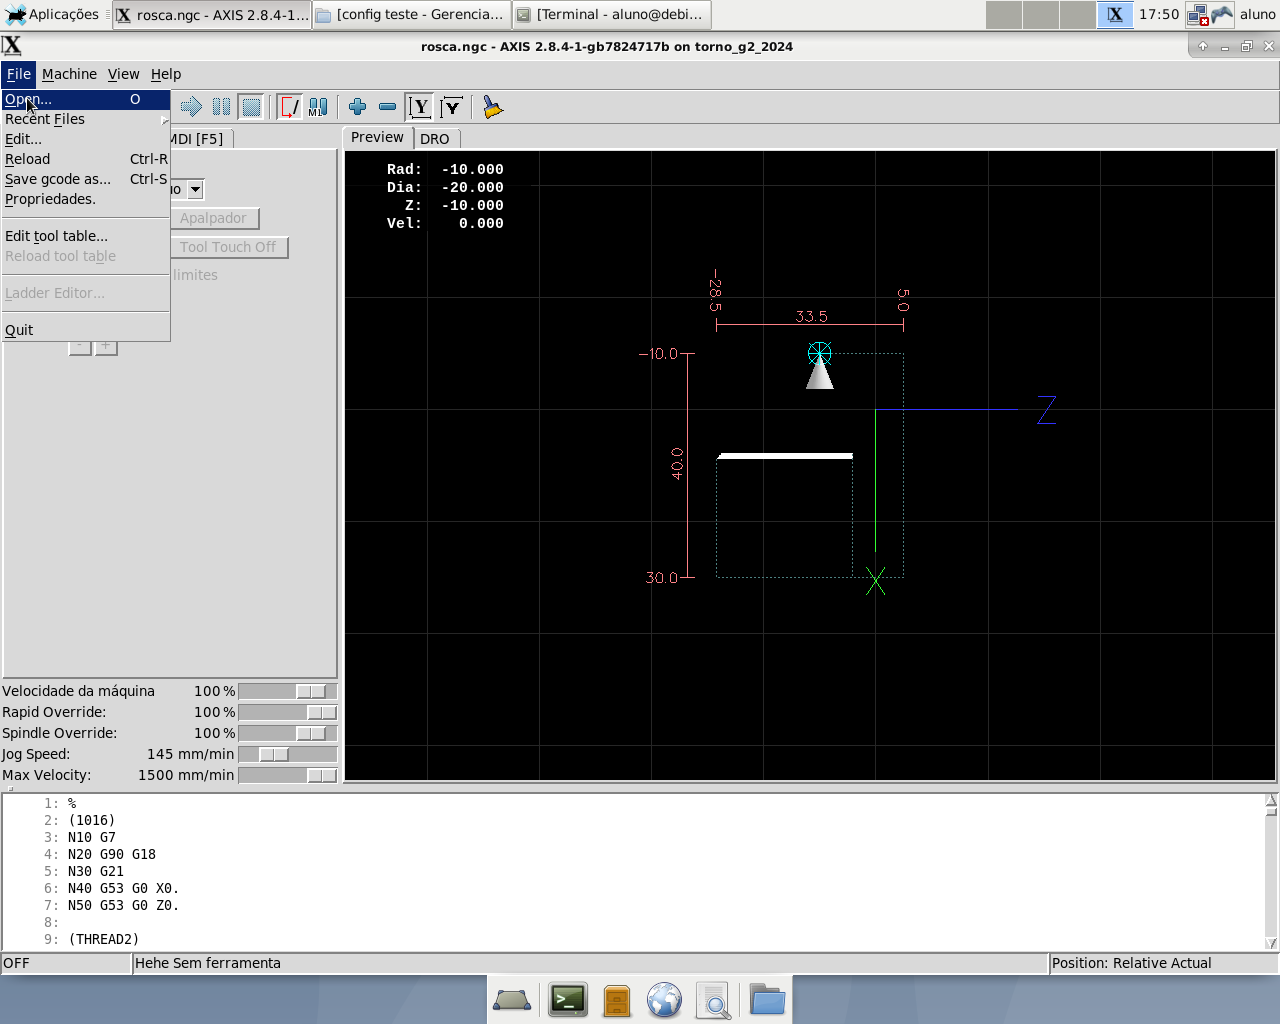
\includegraphics[width=0.95\textwidth]{imagens/Selecao_do_programa2.png}
    \end{center}
    \caption{Programa sendo selecionado}\label{progselec}
\end{figure}

\begin{figure}[H]
    \begin{center}
        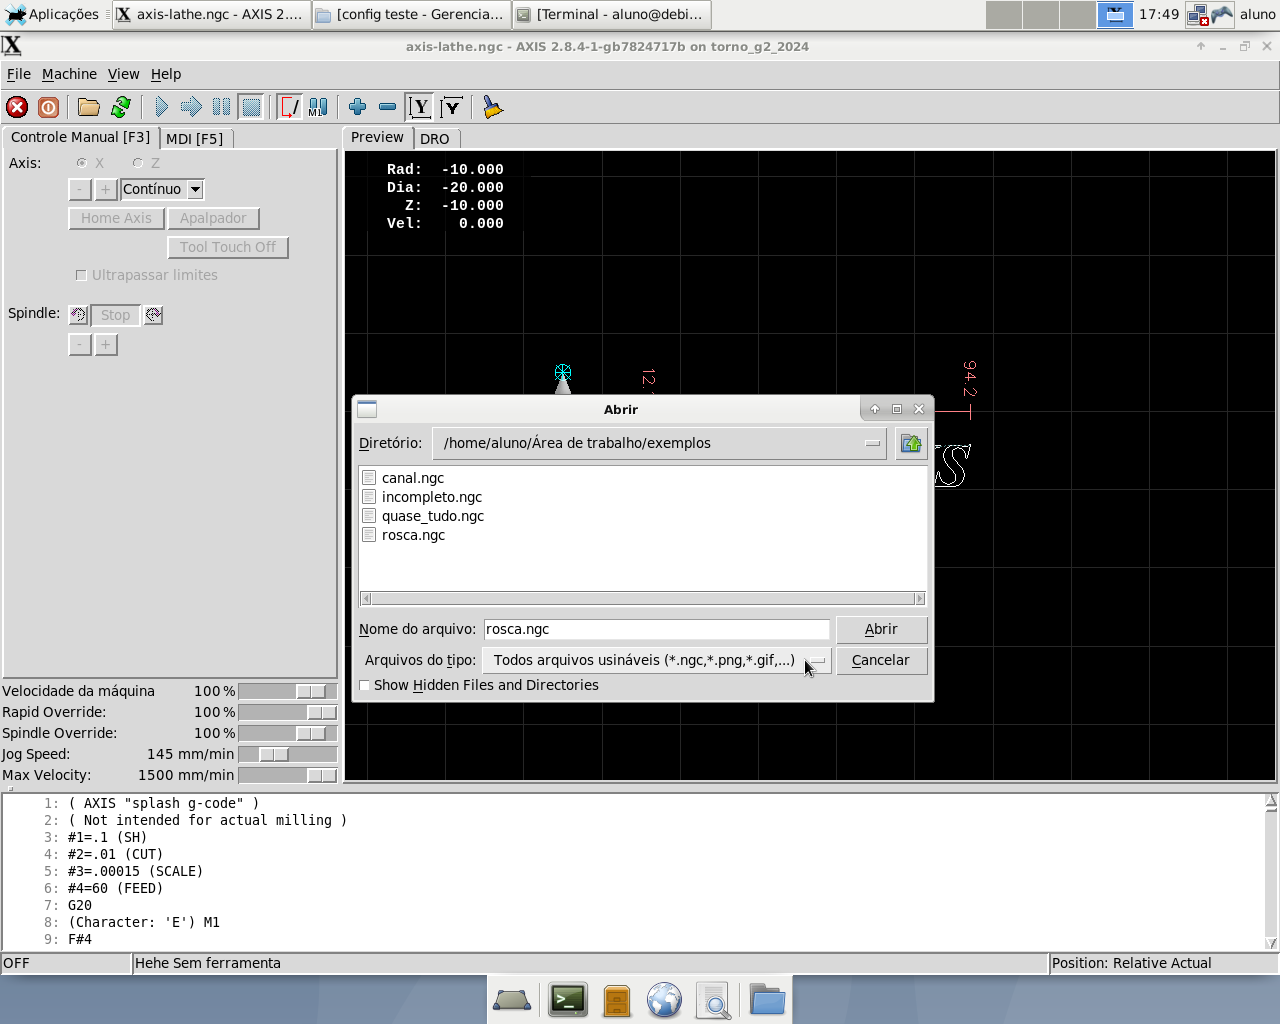
\includegraphics[width=0.95\textwidth]{imagens/Selecao_do_programa.png}
    \end{center}
    \caption{Programa sendo selecionado}\label{progselec2}
\end{figure}

\section{Controles}

O controle manual da máquina é feito através de comandos de teclado que podem ser consultados através da referência rápida do menu "help" do aplicativo do LinuxCNC. Através do uso do qjoypad esse controle pode ser feito através de um Joystick, sendo essa a forma que vai ser avaliada no dia da apresentação final e portanto a forma recomendada. 

Nessa seção são listados todos os comandos programados para funcionar no Joystick, de modo a melhorar a experiência de qualquer usuário seguindo os passos das próximas seções desse manual. 

\begin{itemize}
    \item Direita (d-pad direito, analógico) 
    \item Esquerda (d-pad esquerdo, analógico)
    \item Cima (d-pad acima, analógico)
    \item Baixo (d-pad abaixo, analógico)
    \item Aumentar velocidade (R1) 
    \item Diminuir velocidade (L1)
    \item Selecionar eixo X (L2)
    \item Selecionar eixo Z (R2)
    \item Homing do eixo selecionado (L3, R3, botão 3)
\end{itemize}

\attention O botão 3 é mais consistente que as outras opções de homing.

\attention Apesar de programado no Joystick, fazer o homing de um eixo (que já havia sido referenciado anteriormente) usando o mouse na interface gráfica é equivalente ou até mesmo mais rápido, pois o diálogo de confirmação que é aberto precisa de um clique do mouse. 

\section{Definição do zero peça}

O zero peça é a referência relativa ao zero máquina que passamos ao LinuxCNC para que o mesmo saiba em que coordenadas o material bruto que deve ser torneado está localizado. Podem ser definidos, através de diferentes códigos G, diversos planos de corte, sendo o P0 o plano padrão, em coordenadas absolutas definidas na etapa de homing da máquina.
 
Para definir o zero peça devemos definir um novo plano de corte utilizando a função de \textbf{apalpador} localizada ao lado do botão de homing. Apesar de não ser obrigatório, dê preferência a definir o zero peça usando o plano definido por G54. Abaixo temos uma imagem da função de apalpador sendo utilizada.

\begin{figure}[H]
    \begin{center}
        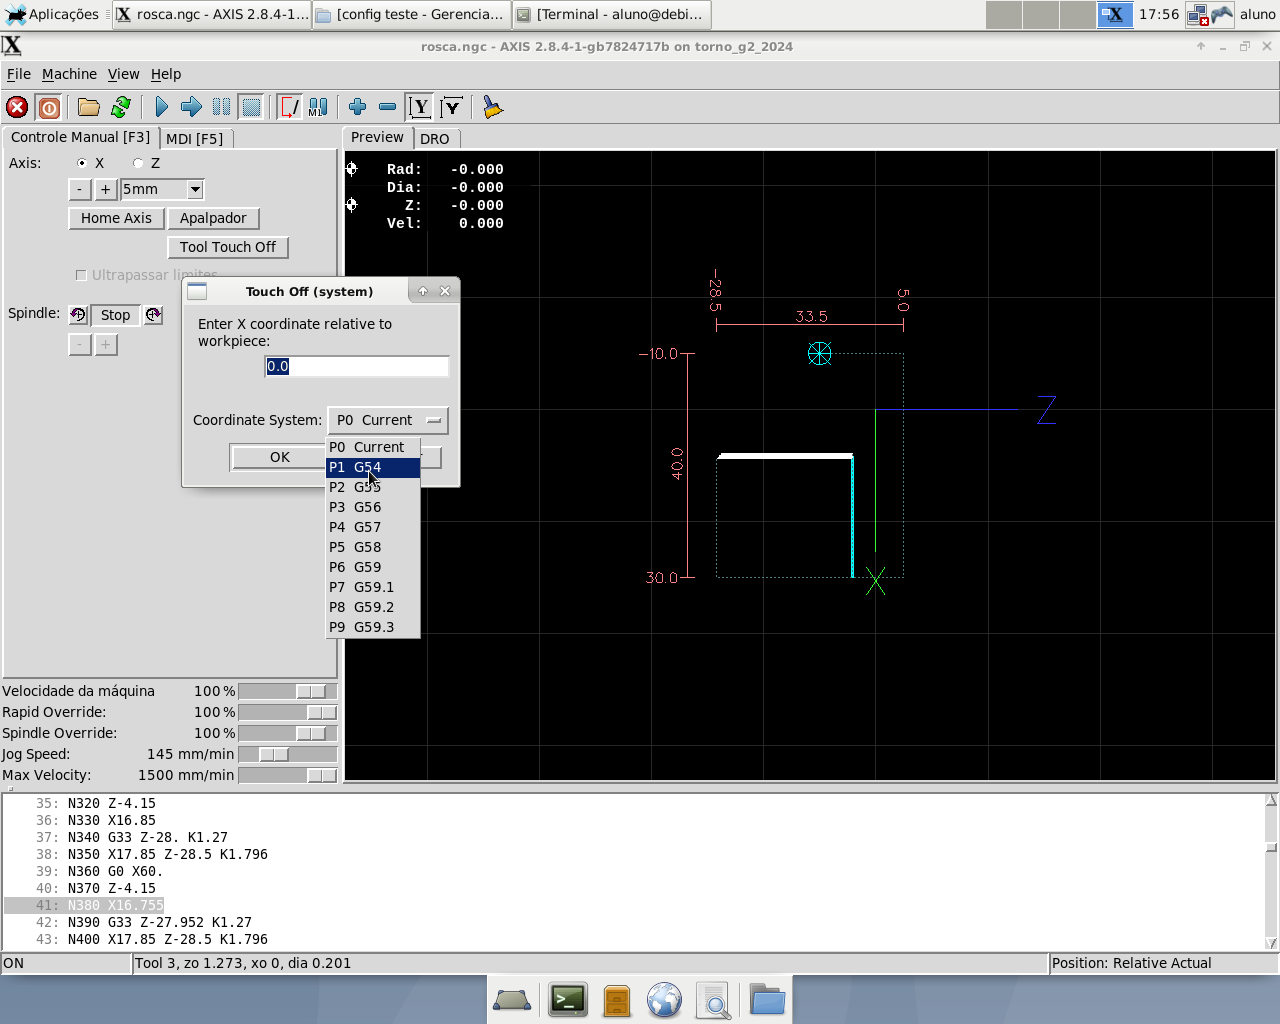
\includegraphics[width=0.95\textwidth]{imagens/Definicao_do_zero_peca_g54.png}
    \end{center}
    \caption{Apalpador sendo utilizado}\label{G54}
\end{figure}


A seguir, uma breve descrição do como usar a função do apalpador para definir o zero peça em cada um dos eixos.

\subsection{Eixo Z}

Leve a ferramenta até a face do tarugo e encoste nela com \textbf{cuidado}, utilizando de preferência o d-pad do Joystick (o teclado também funciona, mas utilizar o Joystick é parte da avaliação). 

Confira se o eixo Z aparece selecionado antes de prosseguir, se não estiver selecione-o de um dos seguintes modos: clicando na opção com o mouse, mudando para o eixo Z usando o L2 do Joystick (recomendado) ou ainda usando o atalho de teclado Z (z maiúsculo).

Clique em apalpador, mantenha o offset em 0, selecione o plano de corte desejado (por favor use o G54 como o padrão para essa operação), clique em "OK". Isso deve mover a imagem da peça na tela, para a nova posição Z que você indicou através desse procedimento.

\attention Use o bom senso ao fazer esse procedimento, controlando a velocidade de aproximação usando os triggers superiores do controle para aumentar ou diminuir a velocidade (L1 diminui a velocidade e R1 aumenta). Consulte o slider na interface gráfica com o nome de "Jog speed" para ver a velocidade com a qual você está avançando (o slider pode ser usado para controlar essa velocidade também, mas novamente é recomendável o uso do Joystick). 

\attention Recomendamos velocidades de aproximação baixas (20 a 50 mm/s) quando prestes a encostar no tarugo de material.

\subsection{Eixo X}

Para esse eixo é preciso conhecer o diâmetro do tarugo que vai ser torneado. Idealmente deve-se fazer um passo manual de desbaste para garantir um diâmetro uniforme ao longo de todo comprimento do tarugo.

De pose dessa informação, leve a ferramenta até a lateral do tarugo e encoste nela com \textbf{cuidado}, utilizando de preferência o d-pad do Joystick (o teclado também funciona, mas utilizar o Joystick é parte da avaliação). 

Confira se o eixo X aparece selecionado antes de prosseguir, se não estiver selecione-o de um dos seguintes modos: clicando na opção com o mouse, mudando para o eixo X usando o R2 do Joystick (recomendado) ou ainda usando o atalho de teclado X (x maiúsculo).

Clique em apalpador, o offset que você deve informar é o diâmetro (assumindo que G7 foi ativado, se não, o raio) do tarugo que você está prestes a tornear, selecione o plano de corte desejado (por favor use o G54 como o padrão para essa operação), clique em "OK". Isso deve mover a imagem da peça na tela, para a nova posição X que você indicou através desse procedimento.

\attention Use o bom senso ao fazer esse procedimento, controlando a velocidade de aproximação usando os triggers superiores do controle para aumentar ou diminuir a velocidade (L1 diminui a velocidade e R1 aumenta). Consulte o slider na interface gráfica com o nome de "Jog speed" para ver a velocidade com a qual você está avançando (o slider pode ser usado para controlar essa velocidade também, mas novamente é recomendável o uso do Joystick). 

\attention Recomendamos velocidades de aproximação baixas (20 a 50 mm/s) quando prestes a encostar no tarugo de material.

\subsection{Preview e DRO}

A interface gráfica do LinuxCNC tem duas seções, Preview e DRO. Preview vem selecionada por padrão e nos mostra o caminho a ferramenta irá percorrer, codificado por cor:

\begin{itemize}
    \item[Amarelo:] marca o caminho percorrido pela ferramenta movida usando o controle manual
    \item[Azul:] caminho programado para a ferramenta onde não é prevista remoção de material
    \item[Branco:] caminho programado para a ferramenta onde é prevista remoção de material
    \item[Vermelho:] marca o caminho percorrido pela ferramenta movida automaticamente seguindo um código G
\end{itemize}

DRO trás varias informações, das quais as mais importantes são a velocidade e a posição do plano de corte G54 em relação as coordenadas X e Z absolutas.

\begin{figure}[H]
    \begin{center}
        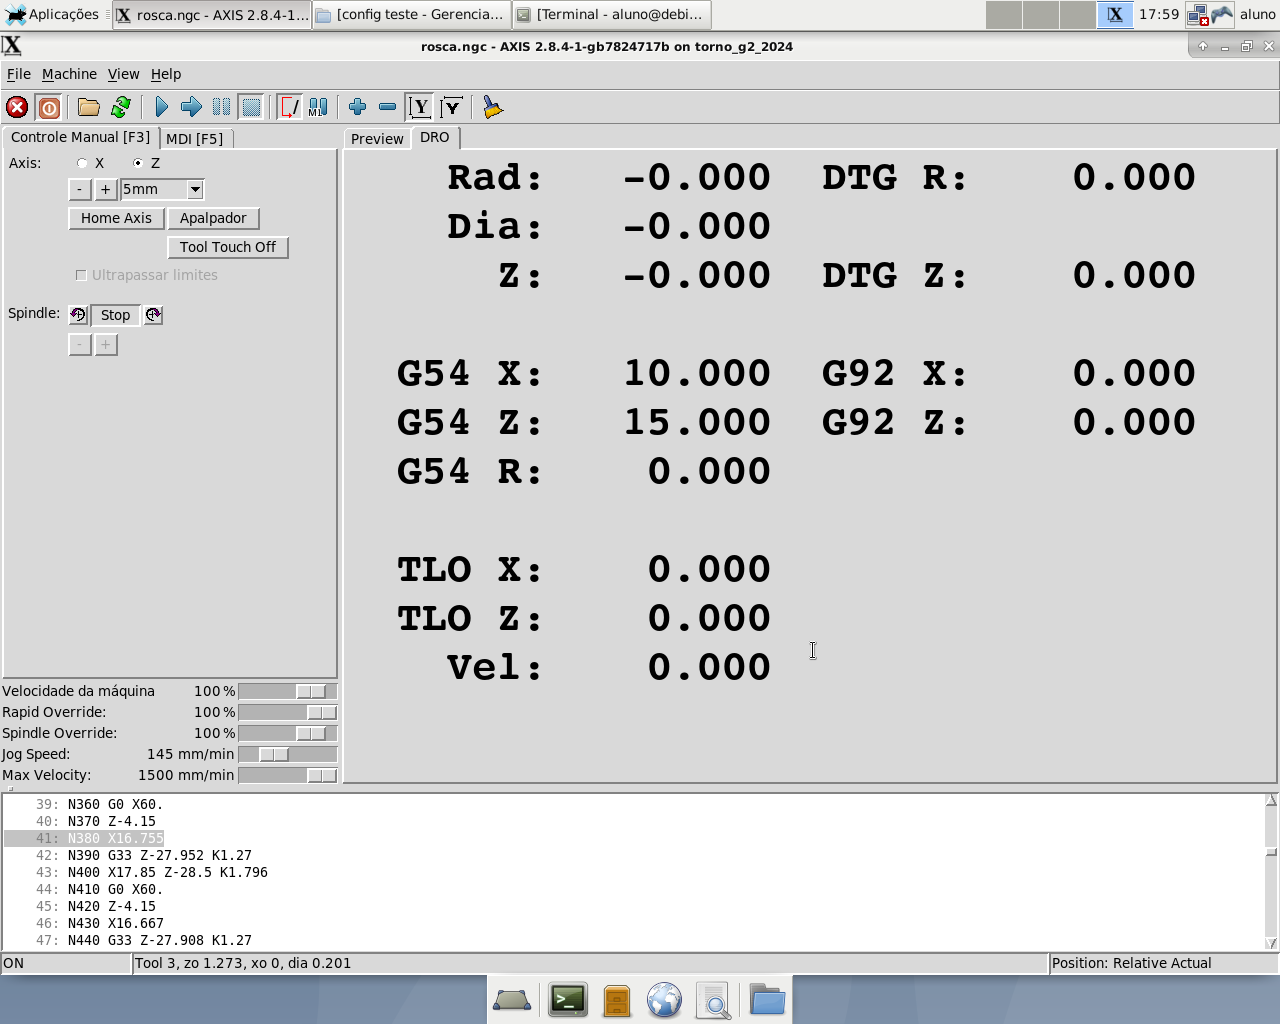
\includegraphics[width=0.95\textwidth]{imagens/configuracao_de_posicao.png}
    \end{center}
    \caption{Interface do DRO}\label{pos}
\end{figure}

\subsection{Testando o zero peça}

Se por alguma razão você estiver em dúvida sobre se o zero peça está definido no lugar certo (centro da face frontal do tarugo), você tem duas opções, refazer a calibração (recomendado), ou usar um comando no MDI para mandar a ferramenta para a coordenada (0, 0) definida em relação a G54 (tome muito cuidado).

Partindo de uma posição segura (ou seja, onde o movimento da ferramenta não tem chance de colidir com o tarugo), um comando como G54 G01 X0. Z0. F100. pode ser executado e se você definiu o zero peça corretamente, não devem haver problemas

\attention Se um procedimento como esse for executado, tenha certeza que você entende o que o comando que você digitar no MDI faz. Além disso, evite velocidades mais altas que a apresentada no exemplo.

\attention Fique atento, se a ferramenta colidir com o tarugo e não parar, esteja pronto para apertar o botão vermelho de emergência localizado na caixa de controle. É melhor ainda se houver outra pessoa pronta para apertar o botão enquanto você manuseia a máquina. 

\section{Executando código G}

Para executar um código G (contido em arquivos .ngc), você deve ter certeza de ter executado todos os passos necessárias anteriormente discutidos neste manual. Além disso, é importante verificar elementos mecânicos da máquina, listados a seguir:

\begin{itemize}
    \item Firmeza do acoplamento da placa de três castanhas ao eixo árvore 
    \item Afiação de todas as ferramentas que serão utilizadas durante a execução do programa 
    \item Distância da placa de três castanhas onde deve ser preso o tarugo, de modo que a peça planejada possa ser executada sem que hajam colisões com as chaves de fim de curso
    \item Firmeza do tarugo uma vez que a placa de castanhas tenha sido apertada
    \item Ajuste das velocidades de rotação do eixo árvore e dos motores de passo
\end{itemize}

É importante salientar que o passo de ajuste de velocidades dos motores de passo é fundamental para evitar avanços muito rápidos que podem lançar o tarugo ou as ferramentas para fora da máquina, o que pode gerar acidentes. Se não foi possível prender o tarugo de forma que sua face posterior toque a placa de castanhas, é quase certo que as velocidades terão de ser reduzidas. Para reduzir as velocidades programadas no código, podemos reduzir tanto a velocidade máxima da máquina, quanto definir um fator de redução (por exemplo se o slider for ajustado para 50\%, o programa roda na metade da velocidade programada no código) através da interface gráfica do LinuxCNC.

Com todas essas precauções tomadas, basta clicar no botão de executar, na interface gráfica do aplicativo. 

\attention Fique muito atento durante a execução de um programa, caso note que algo está dando errado aperte o botão de emergência imediatamente.

\attention Caso o programa pause no meio devido a uma seção no código que exige uma troca de ferramenta manual, troque a ferramenta, refaça os paços para a obtenção do zero peça, e então continue a execução do programa.  

\section{Diagnóstico de problemas}

Aqui apresentaremos alguns problemas comuns encontrados no manuseio da máquina, além de estratégias de diagnóstico para problemas que eventualmente não estejam listados.

\subsection{Problemas de login}

Confira o login e senha anotados por cima do computador, tenha certeza que desativou o caps lock e tente novamente. Se isso não funcionar, tenha certeza de que você fez boot no sistema correto. Para verificar isso, basta reiniciar o computador e esperar que ele selecione o primeiro sistema da lista automaticamente. 

Se nenhuma estratégia funcionar, pode ser preciso realizar a formatação do computador. Consulte o restante do grupo antes de tomar alguma medida nesse sentido.

\subsection{Joystick não consegue mover a máquina}

Verifique que o Joystick está conectado ao computador por meio de uma entrada USB. Caso não esteja, conecte-o e verifique se o Linux foi capaz de detectar o novo dispositivo. Caso não haja detecção, reinicie o computador. 

Verifique que o qjoypad está rodando, olhando se o ícone do aplicativo está presente na barra de tarefas. Caso não esteja, abra um terminal e execute o comando "qjoypad" (note que para continuar ativo o qjoypad precisa que o terminal usado não seja fechado).

Verifique que o modo de controle manual está selecionado na interface gráfica do LinuxCNC, caso contrário os comandos enviados peloJoystick não serão interpretados corretamente.

\attention Não tente usar o controle manual durante uma execução de código G, o LinuxCNC irá ignorar seus comandos manuais e levantar mensagens de erro.

\subsection{Código G não abre}

Tenha certeza que o código que você está tentando abrir tem a extensão usual do LinuxCNC (.ngc). Além disso, verifique a mensagem de erro, podem haver erros na geração do seu código que necessitam de atenção.

Um erro comum é tentar abrir um código G que passa diâmetros em seus parâmetros ao invés de raios, o que pode levar a erro caso você tenha esquecido de ativar o código G7 no MDI. Abaixo, uma imagem de como esse erro pode se apresentar:

\begin{figure}
    \begin{center}
        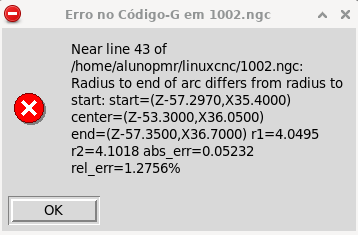
\includegraphics[width=0.95\textwidth]{imagens/erro_g7.png}
    \end{center}
    \caption{Erro devido a não ativação do G7}\label{errog7}
\end{figure}

Se anteriormente seu código funcionava e sem aparente motivo ele não abre mais, você pode estar tentando abrir o arquivo errado por engano, verifique o diretório e o nome do arquivo que você quer abrir.

\subsection{A máquina parou}

Verifique se houveram colisões com as chaves de fim de curso, se for o caso marque a opção "ignorar limites" e leve a máquina para uma posição segura \textbf{com cuidado}. Caso você verifique que a mensagem de erro de colisão esteja presente mas não mas sem uma colisão real, é provável que o motor AC induziu corrente nos fios ligados as chaves de fim de curso, se esse for o caso, refaça a blindagem dos fios. 

Pode ser o caso de uma mera pausa no código para uma troca de ferramenta, se esse for o caso, troque a ferramenta, refaça o referenciamento do zero peça e retome a execução do código.

Se você estiver executando um código atrelado ao sinal do encoder, como por exemplo o código para um rosqueamento, tenha certeza que o motor AC esteja ligado e girando o eixo árvore.

\attention Se o motivo de parada não for aparente, desligue a máquina por precaução.

\subsection{Erros não citados}

Caso você se depare com um erro novo, a melhor estratégia é voltar a um estado inicial seguro. No contexto da operação desse torno, pare a operação imediatamente e reinicie tudo, refazendo todos os passos de preparação necessários.

Se após a reinicialização ainda persistirem erros, verifique as configurações da máquina no Stepconf Wizard (em especial a configuração dos pinos da porta paralela) e os sinais do encoder (encoder.0.phase-A e encoder.0.phase-B) no Halscope

\begin{figure}[H]
    \begin{center}
        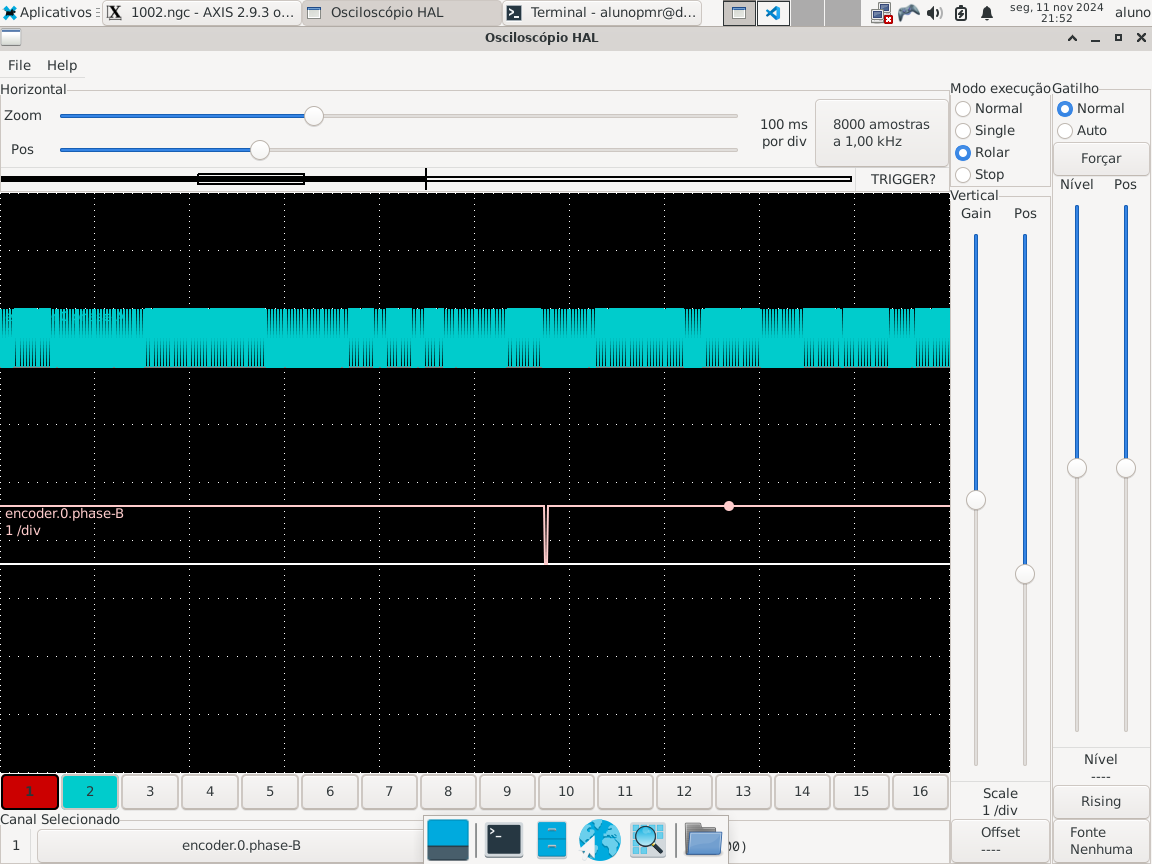
\includegraphics[width=0.95\textwidth]{imagens/halscope.png}
    \end{center}
    \caption{Halscope em uso}\label{halscope}
\end{figure}

\begin{figure}[H]
    \begin{center}
        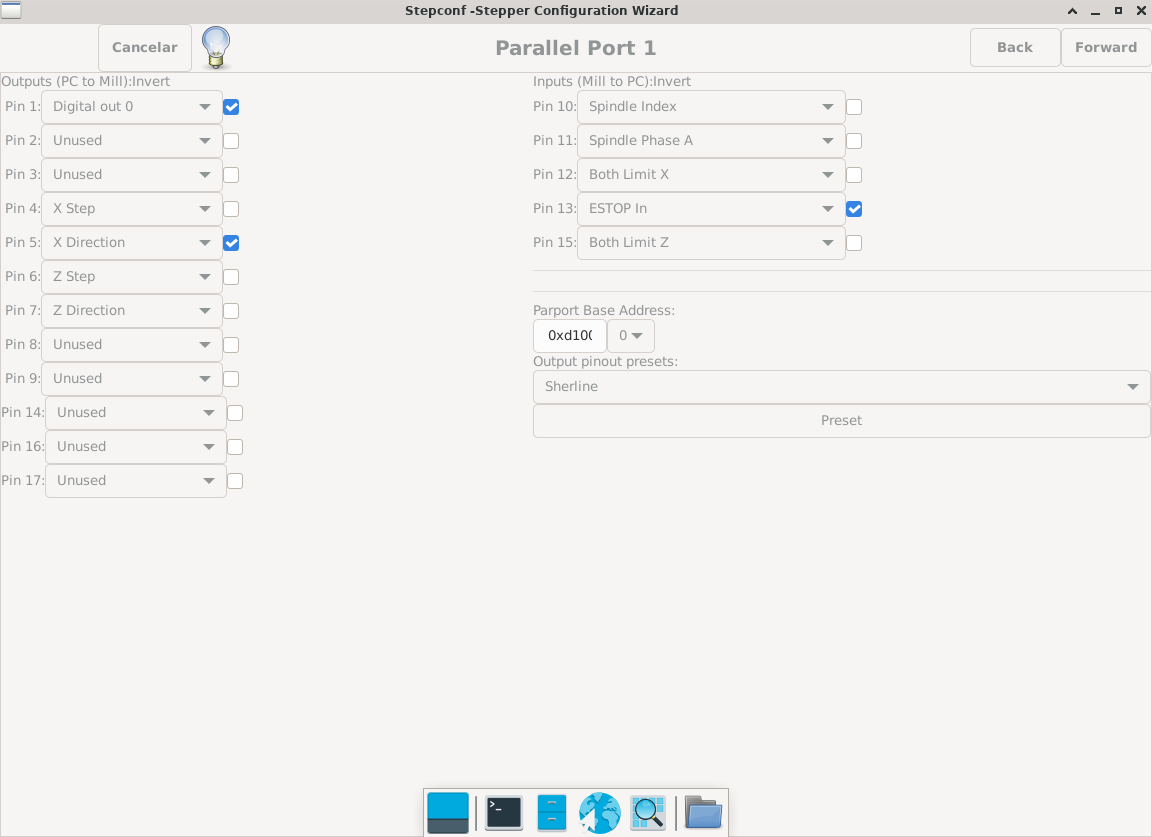
\includegraphics[width=0.95\textwidth]{imagens/stepconf_config.png}
    \end{center}
    \caption{Configuração atual dos pinos}\label{stepconfig}
\end{figure}

\section{Considerações de Segurança}

Operar uma máquina CNC envolve riscos que devem ser mitigados seguindo procedimentos de segurança rigorosos.

\subsection{Uso de Equipamentos de Proteção Individual (EPI)}

\begin{itemize} \item Use óculos de proteção para evitar lesões oculares causadas por partículas. \item Utilize protetores auriculares se o nível de ruído for elevado. \item Evite roupas largas, gravatas, jóias ou qualquer acessório que possa se prender na máquina. \item Prenda cabelos compridos e evite o uso de luvas que possam enroscar. \end{itemize}

\subsection{Procedimentos de Segurança}

\begin{itemize} \item Sempre esteja atento à posição da ferramenta e da peça em relação à máquina. \item Nunca deixe a máquina operando sem supervisão. \item Esteja ciente da localização do botão de parada de emergência e pronto para acioná-lo se necessário. \item Certifique-se de que a área ao redor da máquina está livre de obstáculos e pessoas não autorizadas. \end{itemize}

\subsection{Manutenção Preventiva}

\begin{itemize} 
    \setlength{\itemindent}{-1em}
    \item Inspecione regularmente a máquina em busca de sinais de desgaste ou danos. 
    \item Mantenha a máquina limpa e lubrificada conforme as recomendações do fabricante. 
    \item Relate imediatamente qualquer problema ou anomalia ao responsável técnico. 
\end{itemize}

\section{Manutenção Básica}

A manutenção adequada garante o bom funcionamento da máquina e prolonga sua vida útil.

\subsection{Limpeza}

\begin{itemize} \item Remova os cavacos e resíduos da área de trabalho após cada uso. \item Limpe as guias e componentes móveis com um pano seco ou levemente umedecido. \end{itemize}

\subsection{Lubrificação}

\begin{itemize} \item Aplique lubrificante nas guias e fusos conforme a frequência recomendada. \item Use apenas lubrificantes adequados e indicados pelo fabricante. \end{itemize}

\subsection{Verificações Periódicas}

\begin{itemize} \item Verifique o aperto de parafusos e fixações. \item Teste os sistemas de segurança, como o botão de emergência, regularmente. \item Certifique-se de que os cabos e conexões elétricas estão em bom estado. \end{itemize}

\section*{Glossário}

\begin{description}
	\item[Apalpador] Ferramenta utilizada para definir a posição do zero peça no torno, especialmente para os eixos X e Z.
	
	\item[Caixa de Controle] Unidade de controle elétrico que deve ser conectada à tomada de 220V antes de ligar o computador e o LinuxCNC.
	
	\item[Chaves de Fim de Curso] Sensores que limitam o movimento da máquina para evitar colisões e proteger o operador e o equipamento.
	
	\item[Encoder] Dispositivo que fornece informações de posição e velocidade do eixo árvore, essencial para operações como rosqueamento.
	
	\item[Eixo Árvore] Eixo principal do torno, no qual é fixada a placa de castanhas que segura o tarugo durante a usinagem.

    \item[DRO] Sigla para "Digital Read Out", aba da interface gráfica que exibe informações diversas, como velocidades e posições de planos de corte definidos em relação às coordenadas absolutas.

	\item[G54] Plano de corte padrão no LinuxCNC, geralmente utilizado como referência para definir o zero peça.
	
	\item[Homing] Processo de referenciamento dos eixos do torno (X e Z) para estabelecer uma posição inicial de operação da máquina.
	
	\item[Jog Speed] Controlador de velocidade para movimentos manuais do torno, ajustável através do slider na interface gráfica do LinuxCNC ou pelo Joystick.
	
	\item[Joystick] Dispositivo de controle utilizado para movimentar manualmente os eixos do torno e ajustar a velocidade, substituindo o uso do teclado para melhorar a ergonomia e a segurança.
	
	\item[LinuxCNC] Software de controle numérico que permite a automação do torno e a execução de programas de código G para usinagem.
	
	\item[MDI (Manual Data Input)] Interface de entrada manual de dados do LinuxCNC, usada para inserir comandos G e M diretamente.
	
	\item[Plano de Corte] Referência de coordenadas usada para definir o zero peça. No LinuxCNC, é possível definir múltiplos planos de corte, como o G54.
	
	\item[QJoypad] Aplicativo que permite mapear comandos do teclado para o Joystick, possibilitando o controle do torno por meio desse dispositivo.
	
	\item[Slider de Velocidade] Controlador na interface do LinuxCNC para ajustar a velocidade máxima de execução do código G, ajudando a evitar avanços rápidos demais.
	
	\item[Tarugo] Material bruto preso à placa de castanhas que será usinado conforme o código G carregado no LinuxCNC.
	
	\item[Zero Máquina] Posição de referência absoluta dos eixos, definida pelo processo de homing no LinuxCNC.
	
	\item[Zero Peça] Ponto de referência na peça a partir do qual as coordenadas do código G são baseadas. Definido após o zero máquina e ajustado pelo apalpador.
\end{description}


\end{document}
